\section{Introduction}\label{section introduction}


{\bf Context.} 
Resilience is a key notion for improving safety of unperfect systems and resilience engineering is a paradigm for safety management that focuses on systems coping with complexity and balancing productivity with safety~\cite{challenges}. Some systems are subjects at frequent intervals to accidents, attacks or changes. Think for instance of a supply chain, or an airport’s air trafic control. In such cases, a question that arises is that of whether the system can return to its normal (safe) behavior after an accident or attack
pushed it towards some kind of ‘error state’ and, if it can, whether it can perform the return in a satisfactory timeframe. 
%%%%%%%%
%\alain{fait double emploi avec l'exemple si on le développe ce que je ne suis plus sûr...:  In the exemple of air trafic control, an accident i.e. for instance a delay in the arrival of a plane can lead to conflicts of resolution (i.e. landing) which lead to prompting planes to remain on standby. Since their fuel quantity is limited it is hence pretty important to be able to know that trafic will return to its normal pace quickly enough. We formalize this as the resilience problem. 
%Resilience is then the capacity of a system that fall in a bad set of states to leave this set and to reach a safe set of states. \\
%
%State-resilience only consider bad elements that are reachable from an initial state, while bounded-resilience and $k$-resilience ask whether safe is reachable in a bounded number of step and $k$ or less steps respectively.}


{\bf Home-spaces}
 In 1986, Memmi and Vautherin introduced the notion of home-space~\cite{DBLP:conf/ac/MemmiV86} for a system $\mathscr{S} = (S,\rightarrow )$ with an initial state $s_0$ : a subset $H \subseteq S$ is an \emph{home-space}  if 
%			from all reachable states from $s_0$, it is always possible to reach $H$ 
$\post^*(s_0) \subseteq \pred^*(H)$; it could be easily generalized for two subsets $X,H$ and we say that $H$ is an \emph{home-space for $X$} if $\post^*(X) \subseteq \pred^*(H)$. In 1989, de Frutos Escrig and Johnen proved that the home-space problem (for $X$ a singleton and $H$ a finite union of linear sets with the same period) was decidable for VASS (only published as an internal report). In 2023, Jancar and Leroux proved the decidability of the (complete) semilinear home-space problem ($X$ and $H$ are both semilinear)  in VASS \cite{DBLP:journals/corr/abs-2207-02697}.
%%%%%

{\bf Resiliences.}  
The (general) resilience property for a transition system $\mathscr{S} = (S,\rightarrow )$ and a subset of states $\Safe \subseteq S$ consists of the following: $\mathscr{S}$ is {\em $\Safe$-resilient} if
$S \subseteq \pred^*(\Safe)$. %In the case 
% it
It 
can be stated as an home-space problem : $\mathscr{S}$ is $\Safe$-resilient if $\post^*(S) \subseteq \pred^*(\Safe)$.
Similarly, $\mathscr{S}$ is $\Safe$-state-resilient for an initial state $s_0$ if  
$\post^*(s_0) \subseteq \pred^*(\Safe)$.
We will study three decidability questions for each of type of resilience.
The resilience problem is to decide whether a transition system $\mathscr{S} = (S,\rightarrow )$ is $\Safe$-resilient (for a given subset of states $\Safe \subseteq S$).
The $k$-resilience problem is to decide whether $S \subseteq \pred^{\leq k}(\Safe)$ (for a given $k$) and 
the bounded resilience problem is to decide whether there exists an $k$ such that $\mathscr{S}$ is $\Safe$-$k$-resilient. We adapt these three definitions to state-resilience.


{\bf State of the art.}
In 2016, Prasad and Zuck introduced in  \cite{DBLP:journals/corr/PrasadZ16} interesting definitions and results (without detailed proofs) about resilience in the framework of process algebra. They built the composition of the process and its adversary as a transition system and they gave conditions that insure that the composed transition system is an effective WSTS with both upward and reflexive downward compatibilities (and some other technical conditions). In this framework and under these hypotheses, resilience reduces to coverability which is decidable on WSTS. 
%Since the definition of resilience is only given informally in the introduction as "a process is resilient to an adversary if its observable behaviour in the presence of adversarial action is equivalent to its behaviour in the absence of the adversary", it still remains unclear what is formally resilience.
%%%%%%%%%

In 2021, Ozkan and Würdemann  \cite{DBLP:journals/corr/abs-2108-00889} and Okzan \cite{DBLP:conf/gg/Ozkan22}, in 2022, proved the decidability of the bounded state-resilience problem and the $k$-state-resilience problem for WSTS  with strong compatibility and with the supplementary (strong) hypothesis that there exists an algorithm that computes a finite basis of $\uparrow \post^*(s)$ for all state $s$ (called effective 
$\uparrow$ $\post^*$ basis) and with $\Safe=\uparrow \Safe$, (hence $\Bad$ is downward-closed).
%		(even though \cite{DBLP:conf/gg/Ozkan22} also discuss, albeit briefly, the other possible cases). 
%		The paper of Prasad and Zuck \cite{DBLP:journals/corr/PrasadZ16} is not quoted by Ozkan and Würdemann.

Remark that the reflexive downward compatibility (of an effective WSTS) hypothesis in  \cite{DBLP:journals/corr/PrasadZ16} implies the existence of an algorithm that computes a finite basis of $\uparrow \post^*(s)$ for all state $s$; this provides a way to use \cite{DBLP:journals/corr/abs-2108-00889} for proving the announced result by Prasad and Zuck.
However, neither Prasad \& Zuck nor Ozkan \& Würdemann established the strong relation between resilience and the home-space property.
%%%%%%%%%
%





% {\bf FSTTCS 2033  Submission deadline: July 14, 2022 AoE (firm) Notification to authors: September 16, 2022}

% trop d'hypotheses trop fortes sur les WSTS
\noindent
{\bf Our contributions}
\begin{itemize}
%\item We investigate and expand upon the notion of state-resilience ~\cite{DBLP:journals/corr/PrasadZ16,DBLP:journals/corr/PrasadZ16,DBLP:journals/corr/abs-2108-00889,DBLP:conf/gg/Ozkan22} and we study three decidability questions for each of type of resilience. We remark that it is an instance of the home-space problem~\cite{DBLP:journals/corr/abs-2207-02697,memmi2023invariants}.

\item Surprinsingly, the general undecidability statements about resilience were not known neither proved. We show that resilience and { State-resilience} problems are both undecidable for WSTS with strong compatibility. 
% \alain{harminiser les notations des pbs { State-resilience} ou  State-resilience ?}
% \mathieu{je pense dans l'intro on peut conserver State-resilience et par contre une fois le probleme de {\ State-resilience} proprement défini c'est cette notation qu'il faudrait utiliser}
%Moreover, state-resilience,
%bounded-state-resilience and
% $k$-state-resilience
%are undecidable for WSTS with strong compatibility having an effective pred-basis. 
Moreover, { State-resilience},
{ Bounded-state-resilience} and
{ $k$-state-resilience}
are undecidable for strongly upward-compatible WSTS with effective pred-basis
when
$\Safe=\uparrow \Safe$. We made a reduction of zero-reachability in reset-VASS to {\ State-resilience} in reset-VASS.


\item The three resilience problems are decidable for completion-post-effective $\omega^2$-WSTS with strong compatibility and $\Safe = \uparrow \Safe$.


\item The resilience problem is decidable for ideal-effective WSTS with 
$\Safe=\downarrow \Safe$
and
the additional hypothesis that
for all downward-closed set $D \subseteq S$, the set $\pred^*(D)$ is downward-closed.
%
%%%

\item We generalize the main theorem of \cite{DBLP:journals/corr/abs-2108-00889,DBLP:conf/gg/Ozkan22} by relaxing the strong compatibility hypothesis.
%: {\ State-resilience} is still decidable for 
% WSTS with effective 
%$\uparrow$ $\post^*$ basis
%when
%$\Safe=\uparrow \Safe$
We also show that removing the effective 
$\uparrow$ $\post^*$ basis hypothesis leads to undecidability. We extend and prove the main result in  \cite{DBLP:journals/corr/PrasadZ16} : the three state-resilience problems are decidable for ideal-effective WSTS with downward and upward compatibilities ({ $k$-state-resilience} and { bounded-state-resilience} are decidable for ideal-effective WSTS with strong downward compatibility).
%

\item We study the resilience problems for VASS and variations of VASS where most of the resilience problems are shown decidable.
\end{itemize}


 
\begin{center}
	\begin{figure}
			\hspace{2cm}
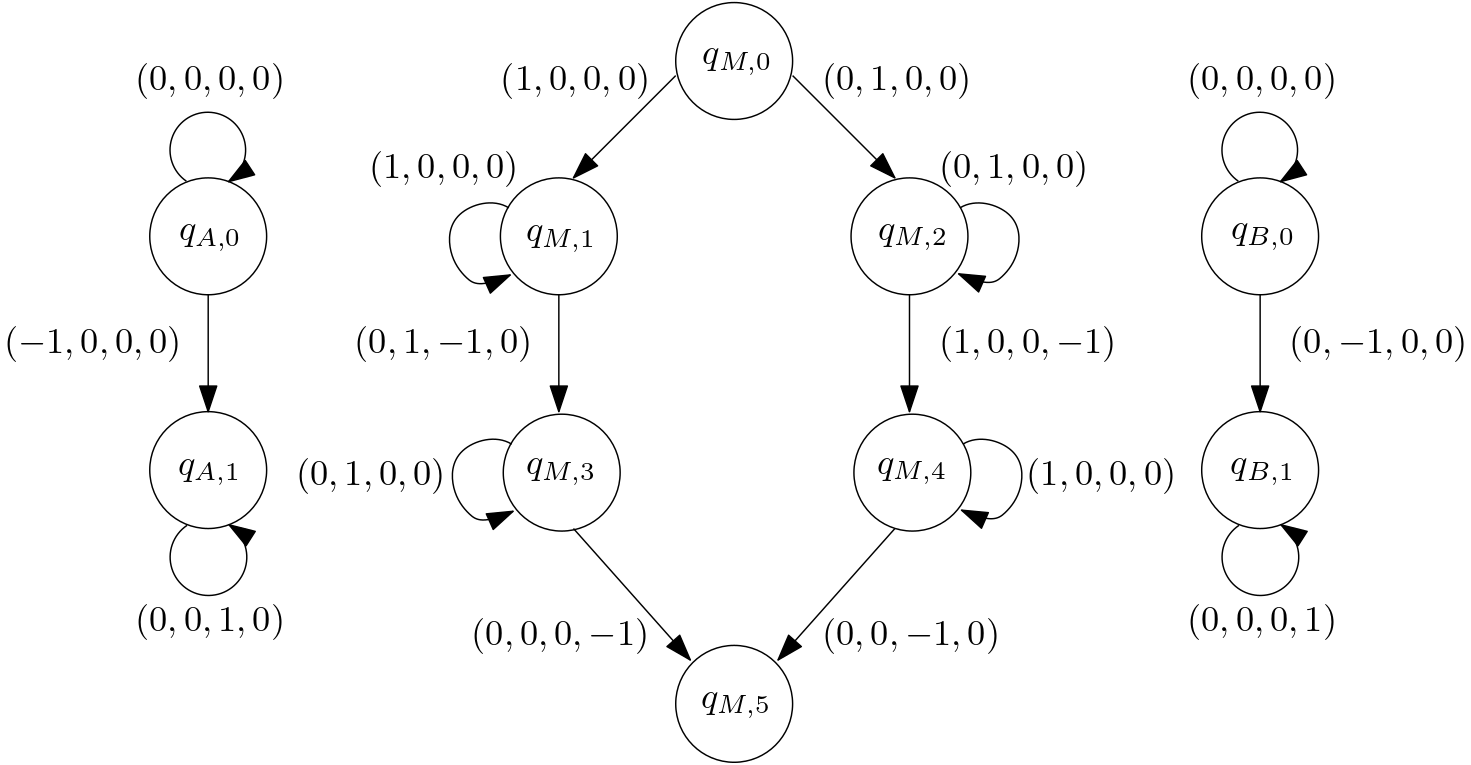
\includegraphics[width=0.65\textwidth]{FigureB}
	\caption{A lossy (distributed) VASS with three subsystems and four counters. Leftmost and rightmost subsystems $A$ and $B$ represent aircrafts attempting to land and staying on stand-by in the air while they haven't received permission to land, while the middle one $C$ represents the control tower managing the aircrafts landings so that only one aircraft at a time is allowed for landing. Arrows represent control-transitions. Unlabelled arrows do not modify counter values.}
					\label{air control}
	\end{figure}
\end{center}

\begin{example}\label{Example}
{(\bf Flight Controller System).}
Consider the (distributed) VASS in Figure~\ref{air control}. It models a scenario in which two aircrafts want to land in an airport at the same time. 
The VASSs $A$ on the left and $B$ on the right represent the aircrafts attempting to land, while the middle one $M$ represents the control tower. The control tower can communicate information to the aircrafts using 
% channels $c_1$ and $c_2$, and these in turn can send messages to the control tower using 
the first two shared counters, and these in turn can send messages to the control tower
using the last two shared counters. 
% respectively channel $c_3$ and $c_4$. 
% Remark channels $c_3$ and $c_4$ have a unary alphabet in the exemple and therefore can be seen as counters. 

Safety requires that only one aircraft at a time attempts to land. The role of the control tower is to ensure this;
there are two possible choices: aircraft $A$ waits for aircraft $B$ to land
or vice-versa. To make its choice known to the aircrafts, the control tower will use the counters. 
We assume that the VASS is
lossy;  \alain{à quoi sert cette phrase ?Lossiness will be represented by using transitions decreasing any counter by one from every state.}
% We ask however that the system is not too lossy. We add the condition that for every prefix of an execution, the number of ``lossiness transition'' for a counter is less than nine tenth of the number of transitions incrementing said counter.
The safe states would be ones where the aircrafts have both landed, i.e.
$\Safe = \{(q_{A,1}, q_{M,i}, q_{B,1})(\textbf{v}) \mid \textbf{v} \in \N^4, i \in \N\}$%, and $\Bad$ is the complement of $\Safe$. 
.
Resilience here expresses that the aircrafts will both land, while $k$-resilience is the property insuring that they will do so in at most $k$ steps. 
%$k$-resilience is of interest since in general we want to ensure the safe space will 
%be reached in
%the least amount of steps possible. 
In this exemple, aircrafts cannot simply wait in the air an unbounded amount of time: here, $8$-resilience hold but $8$-resilience don't.\alain{expliquer}
\end{example}

% contrôle de trafic aérien, perturbation dans le planning → Bad (par exemple, trop d’avions qui cherchent à atterir en même temps et qui doivent être mis en stand-by au dessus de l’aéroport?) → Safe (trafic fluide à nouveau). K-résilience important car les avions peuvent pas rester indéfiniment en stand-by (re : le carburant est un réactif limitant) 



